\documentclass[letterpaper,11pt,oneside,reqno]{article}

%%%%%%%%%%%%%%%%%%%%%%%%%%%%%%%%%%%%%%%%%%%%%%%%%%%%%%%%%%%%

\usepackage[pdftex,backref=page,colorlinks=true,linkcolor=blue,citecolor=red]{hyperref}
\usepackage[alphabetic,nobysame]{amsrefs}

%%%%%%%%%%%%%%%%%%%%%%%%%%%%%%%%%%%%%%%%%%%%%%%%%%%%%%%%%%%%
%main packages
\usepackage{amsmath,amssymb,amsthm,amsfonts,mathtools}
\usepackage{graphicx,color}
\usepackage{upgreek}
\usepackage[mathscr]{euscript}

%equations
\allowdisplaybreaks
\numberwithin{equation}{section}

%tikz
\usepackage{tikz}
\usetikzlibrary{shapes,arrows,positioning,decorations.markings}

%conveniences
\usepackage{array}
\usepackage{adjustbox}
\usepackage{cleveref}
\usepackage{enumerate}
\usepackage{datetime}

%paper geometry
\usepackage[DIV=12]{typearea}

%%%%%%%%%%%%%%%%%%%%%%%%%%%%%%%%%%%%%%%%%%%%%%%%%%%%%%%%%%%%
%draft-specific
\synctex=1
% \usepackage{refcheck,comment}

%%%%%%%%%%%%%%%%%%%%%%%%%%%%%%%%%%%%%%%%%%%%%%%%%%%%%%%%%%%%
%this paper specific
\newcommand{\ssp}{\hspace{1pt}}

%%%%%%%%%%%%%%%%%%%%%%%%%%%%%%%%%%%%%%%%%%%%%%%%%%%%%%%%%%%%
\newtheorem{proposition}{Proposition}[section]
\newtheorem{lemma}[proposition]{Lemma}
\newtheorem{corollary}[proposition]{Corollary}
\newtheorem{theorem}[proposition]{Theorem}
%%%%%%%%%%%%%%%%%%%%%%%%%%%%%%%%%%%%%%%%%%%%%%%%%%%%%%%%%%%%
\theoremstyle{definition}
\newtheorem{definition}[proposition]{Definition}
\newtheorem{remark}[proposition]{Remark}
\newtheorem{example}[proposition]{Example}
%%%%%%%%%%%%%%%%%%%%%%%%%%%%%%%%%%%%%%%%%%%%%%%%%%%%%%%%%%%%

\begin{document}
\title{Lectures on Random Matrices
(Spring 2025)
\\Lecture 1: Moments of random variables and random
matrices}


\date{Monday, January 13, 2025\footnote{\href{https://lpetrov.cc/rmt25/}{\texttt{Course webpage}}
$\bullet$ \href{https://lpetrov.cc/rmt25/rmt25-notes/rmt2025-l01.tex}{\texttt{TeX Source}} 
$\bullet$
Updated at \currenttime, \today}}



\author{Leonid Petrov}


\maketitle



\section{Recall Central Limit Theorem}

We begin by establishing the necessary groundwork for understanding and proving 
the Central Limit Theorem. The theorem's power lies in its remarkable universality: 
it applies to a wide variety of probability distributions under mild conditions.

\begin{definition}
A sequence of random variables $\{X_i\}_{i=1}^{\infty}$ is said to be 
\emph{independent and identically distributed (i.i.d.)} 
if:

\begin{itemize}
    \item Each $X_i$ has the same probability distribution as every other $X_j$, for all $i, j$.
    \item The variables are mutually independent, meaning that for any finite subset $\{X_1, X_2, \dots, X_n\}$, the joint distribution factors as the product of the individual distributions:
    \[
			\operatorname{\mathbb{P}}(X_1 \leq x_1, X_2 \leq x_2, \dots, X_n \leq x_n) 
			=
			\operatorname{\mathbb{P}}(X_1 \leq x_1) 
			\operatorname{\mathbb{P}}(X_2 \leq x_2) \cdots \operatorname{\mathbb{P}}(X_n \leq x_n).
    \]
\end{itemize}
\end{definition}

\begin{theorem}[Classical Central Limit Theorem]
	Let $\{X_i\}_{i=1}^{\infty}$ be a sequence of i.i.d. random variables with finite mean $\mu = \operatorname{\mathbb{E}}[X_i]$ and finite 
	variance $\sigma^2 = \operatorname{\mathrm{Var}}(X_i)$. 
	Define the normalized sum
\[
Z_n = \frac{1}{\sqrt{n}} \sum_{i=1}^n \left(X_i - \mu\right).
\]
Then, as $n \to \infty$, the distribution of $Z_n$ converges in distribution to a normal random variable with mean $0$ and variance $\sigma^2$, i.e.,
\[
Z_n \xrightarrow{d} \mathcal{N}(0, \sigma^2).
\]
\end{theorem}
Convergence in distribution means 
\begin{equation}
	\label{eq:conv-in-dist}
	\lim_{n \to \infty} \operatorname{\mathbb{P}}(Z_n \leq x) = \operatorname{\mathbb{P}}(Z \leq x)
		= \int_{-\infty}^x \frac{1}{\sqrt{2\pi \sigma^2}}\ssp e^{-\frac{t^2}{2\sigma^2}} \, dt
	\qquad 
	\text{for all } x \in \mathbb{R},
\end{equation}
where $Z \sim \mathcal{N}(0, \sigma^2)$ is the Gaussian random variable.

\begin{remark}
	For a general random variable instead of
	$Z\sim \mathcal{N}(0, \sigma^2)$, the convergence in distribution
	\eqref{eq:conv-in-dist} holds only for $x$ at which the cumulative distribution function of $Z$ is continuous.
	Since the normal distribution is absolutely continuous (has density), the convergence holds for all $x$.
\end{remark}
\begin{figure}[htpb]
	\centering
	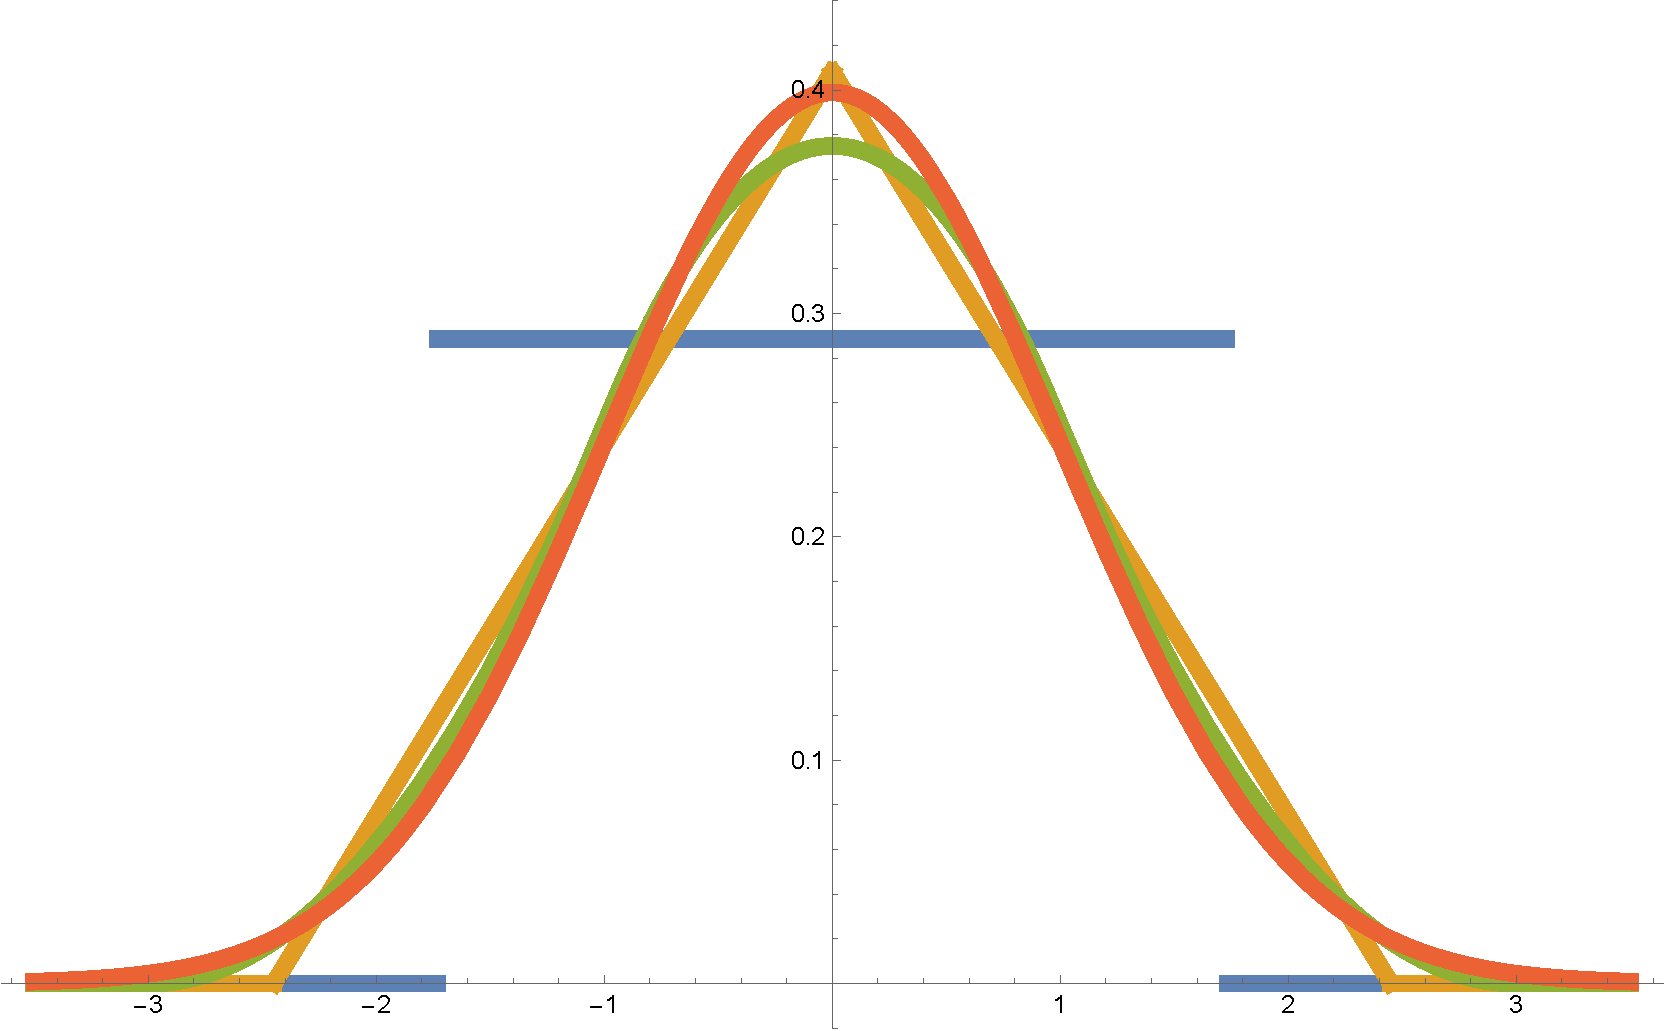
\includegraphics[width=0.5\textwidth]{./pictures/uniform_pdfs.pdf}
	\caption{Densities of $U_1$, $U_1+U_2$, $U_1+U_2+U_3$ (where $U_i$ are iid uniform on $[0,1]$), 
		and $\mathcal{N}(0,1)$, 
		normalized to have the same mean and variance.}
	\label{fig:uniform_pdfs}
\end{figure}

\begin{example}
Let $\{X_i\}_{i=1}^{\infty}$ be a sequence of i.i.d. Bernoulli random variables with parameter $p$, meaning that each $X_i$ takes the value $1$ with probability $p$ and $0$ with probability $1 - p$. The mean and variance of each $X_i$ are given by:
\[
	\mu = \operatorname{\mathbb{E}}[X_i] = p, \quad \sigma^2 = \operatorname{\mathrm{Var}}(X_i) = p(1 - p).
\]
We also have the distribution of $X_1+\cdots+X_n$:
\begin{equation*}
	\operatorname{\mathbb{P}}\left( X_1+ \cdots + X_n = k \right) = \binom{n}{k} p^k (1-p)^{n-k},
	\qquad k = 0, 1, \ldots, n.
\end{equation*}

\colorbox{yellow}{\parbox{.7\textwidth}{local CLT via Stirling}}

\end{example}









































\bibliographystyle{alpha}
\bibliography{bib}


\medskip

\textsc{L. Petrov, University of Virginia, Department of Mathematics, 141 Cabell Drive, Kerchof Hall, P.O. Box 400137, Charlottesville, VA 22904, USA}

E-mail: \texttt{lenia.petrov@gmail.com}


\end{document}
